\documentclass[cmptslides]{cmpt280-slidesandsolutions}


\date{}
\title{Tutorial 1}
\subtitle{Assignment 1, lib280, and you!}

\institute{University of Saskatchewan}
\author{Mark G. Eramian; G. Scott Johnston}


\newcommand{\cc}[1]{\texttt{#1}}
\newcommand{\lib}{\texttt{lib280}}
\newcommand{\libasn}{\texttt{lib280-asn1}}

\newcommand{\BlistJ}{\texttt{BilinkedList280.java}}
\newcommand{\BiterJ}{\texttt{BilinkedIterator280.java}}

\newcommand{\Blist}{\texttt{BilinkedList280}}
\newcommand{\Llist}{\texttt{LinkedList280}}
\newcommand{\Biter}{\texttt{BilinkedIterator280}}
\newcommand{\Liter}{\texttt{LinkedIterator280}}
\newcommand{\Linter}{\texttt{LinearIterator280}}
\newcommand{\Binter}{\texttt{BilinearIterator280}}



\begin{document}

\maketitle


\frame{
\frametitle{The Plan}

\begin{enumerate}
\item Introduction to List classes in lib280.
\item Examples
	\begin{itemize}
	\item How to use a \texttt{LinkedList280} and \texttt{LinkedIterator280}.
	\end{itemize}
\item Go over Assignment 1 so that everything is clear. 
	\begin{itemize}
	\item Review the tasks to be completed on Assignment 1. 
	\item Run through the tutorial on importing lib280 into IntelliJ and setting up a project to use it.
	\end{itemize}


\end{enumerate}

}




%\frame{
%\frametitle{Background}
%
%\begin{itemize}
%	\item \libasn{}
%	\item Make sure to look at the ``self-guided tutorial'' on how to include it.
%		\begin{enumerate}
%		\item Import to Eclipse
%		\item Make your own project include that project.
%		\end{enumerate}
%\end{itemize}
%
%}


\part{Introduction to List classes in lib280.}
\frame{
\partpage
}

\frame{
\frametitle{Singly- and Doubly- Linked List Classes in \lib{}}
%\framesubtitle{The Diagram}
%
%The UML diagram below shows the class hierarchy you'll be working with in this assignment.  It may look a bit daunting at first, but you'll soon see it's not that complicated.  In essence, there are four pairs of classes/interfaces (denoted by light blue boxes\footnote{The light blue boxes in the UML diagram are only to show the pairs of classes that serve the same roles for singly-/doubly-linked lists and do not represent any actual grouping within \texttt{lib280}.  All of the pictured classes are in the same package within \texttt{lib280}.}). and in each pair, one is for a singly-linked list and one for a doubly-linked list. The class/interface of each pair that pertains to doubly linked lists extends the class/interface related to singly linked lists.
%
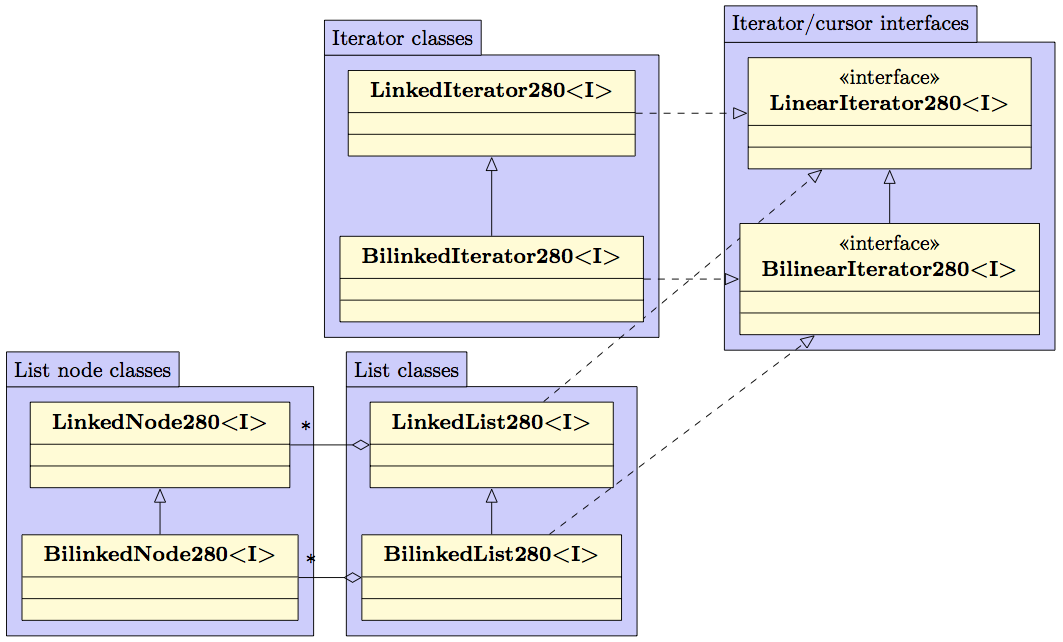
\includegraphics[width=\linewidth]{figures/hierarchy.png}

(Remember: here, purple packages are for grouping, not packages.)

}


\frame{
\frametitle{Singly- and Doubly- Linked List Classes in \lib{}}
\framesubtitle{List Nodes}
\begin{columns}
\column{0.5\textwidth}
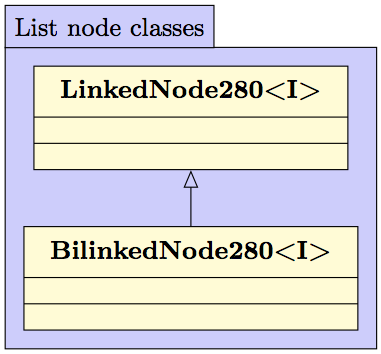
\includegraphics[width=\columnwidth]{figures/nodes.png}
\column{0.5\textwidth}
\begin{itemize}
	\item Each one stores an object from generic class \texttt{I}. 
	\item A \texttt{BilinkedNode280} is a little bit more than a \texttt{LinkedNode280}.
	\item Includes a previous (\texttt{prev}) reference in addition to the \texttt{next} node reference in \texttt{LinkedNode280}; also accessor and mutator for the \texttt{prev} reference.
\end{itemize}
\end{columns}
}


\frame{
\frametitle{Singly- and Doubly- Linked List Classes in \lib{}}
\framesubtitle{Lists}
\begin{columns}
\column{0.5\textwidth}
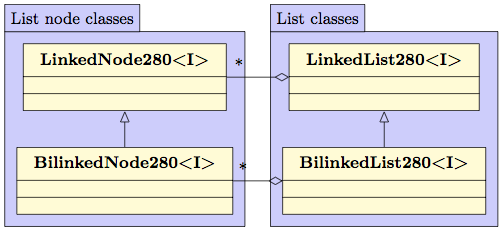
\includegraphics[width=\columnwidth]{figures/nodes_lists.png}
\column{0.5\textwidth}
\begin{itemize} 
	\item Lists are collections of nodes.
	\item A \textit{BilinkedList280} is a little bit more than a LinkedList.  E.g. includes \texttt{tail} reference not in \texttt{LinkedList280}.
	\item Some inherited methods must be overridden in \textit{BilinkedList280} to keep track of \texttt{tail} and node \texttt{prev} pointers.
\end{itemize}
\end{columns}
}

\frame{
\frametitle{Singly- and Doubly- Linked List Classes in \lib{}}
\framesubtitle{Iterator/Cursor Interfaces}
\begin{columns}
\column{0.5\textwidth}
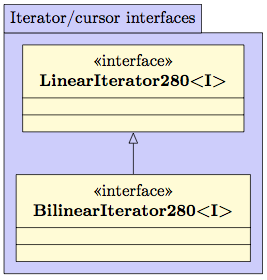
\includegraphics[width=\columnwidth]{figures/interfaces.png}

(Actually in the \texttt{lib280.base} package.)
\column{0.5\textwidth}
An interface is a specific pattern of behaviour. 
\begin{itemize}[itemsep=1pt,topsep=0pt]
	\item \cc{boolean before()}
	\item \cc{void goBefore()}
	\item \cc{boolean after()}
	\item \cc{void goAfter()}
	\item \cc{void goFirst()}
	\item \cc{void goForth()}
	\item \cc{I item()}
	\item \cc{boolean itemExists()}
\end{itemize}

\vspace{.5em}
\texttt{BlinearIterator280} adds:
\begin{itemize}[itemsep=1pt,topsep=0pt]
	\item \cc{void goLast()}
	\item \cc{void goBack()}
\end{itemize}
\end{columns}
}




\newcommand{\str}[1]{\textit{\textbf{\underline{#1}}}}

\frame{
\frametitle{Singly- and Doubly- Linked List Classes in \lib{}}
\framesubtitle{Iterators}
\begin{columns}
\column{0.5\textwidth}
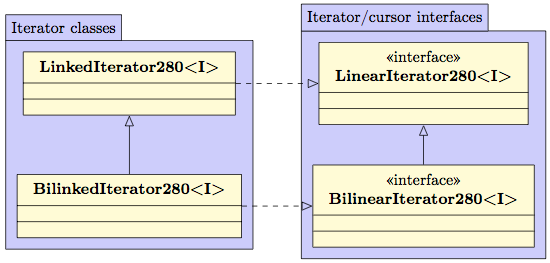
\includegraphics[width=\columnwidth]{figures/iterators.png}
\column{0.5\textwidth}
\begin{itemize} 
	\item \texttt{LinkedIterator280} and \texttt{BilinkedIterator280} implement the linear iterator interfaces.

%	\item Interfaces aren't real things.  
%	\item Iterators: real things that actually iterate.
%	\item (\str{Classes} that can be \str{instantiated} as \str{objects}, 
%		instead of \str{interfaces} that classes \str{implement}.)
\end{itemize}
\end{columns}
}



\frame{
\frametitle{Singly- and Doubly- Linked List Classes in \lib{}}
\framesubtitle{Cursors}
\begin{columns}
\column{0.4\textwidth}
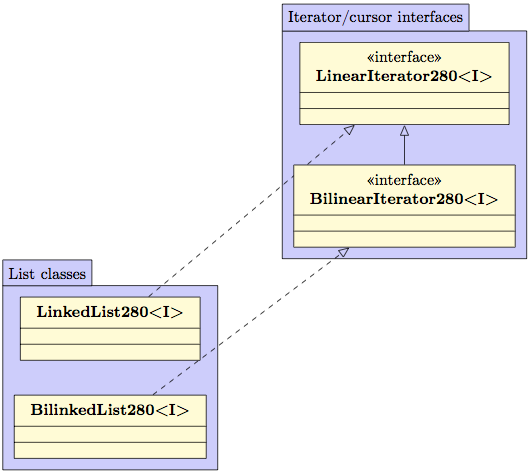
\includegraphics[width=\columnwidth]{figures/interfaces_lists.png}
\column{0.6\textwidth}
The list classes can have cursors by implementing the same linear iterator interfaces. 

\begin{itemize} 
	\item \Blist{} directly implements \Binter{}.
	\item \Llist{} implements \Linter{}
\end{itemize}
Thus the linked lists in lib280 have both cursors and iterators.
\end{columns}
}







\frame{
\frametitle{Iterators}

\begin{block}{Reminder:}
Iterators provide the same functionality as a container ADT that has a cursor, but they are separate objects from the container.  This allows us to record a cursor position that is different and independent from the position recorded by the container's internal cursor.
\end{block}
}



\frame{
\frametitle{Cursors vs. Iterators}
\framesubtitle{Uses of Cursors}

\begin{itemize}
\item Insert an element \texttt{y} immediately before an element \texttt{x} already in the list:
	\begin{enumerate}[itemsep=2pt,topsep=2pt]
	\item \texttt{search(x)} to find \texttt{x}
	\item \texttt{insertBefore(y)} to add \texttt{y} right after \texttt{x}
	\end{enumerate}
\item Delete an item from the list:
	\begin{enumerate}[itemsep=2pt,topsep=2pt]
	\item \texttt{search(x)} to find \texttt{x} in the list
	\item if \texttt{itemExists()} then \texttt{deleteItem()} to delete \texttt{x}	\end{enumerate}
\end{itemize}
These tasks use the cursor to do something to the list based on the position of the cursor.  The internal representation of position is \textbf{abstracted}.  The \texttt{ArrayedList280} classes uses the same cursor interface, so positions within a list can be manipulated in exactly the same way for both classes, despite the differences in the internal data structure.
}



\frame{
\frametitle{Cursors vs. Iterators}
\framesubtitle{Iterators}


An iterator is external, for accessing data only indirectly.
	\begin{itemize}
		\item Example uses:
			\begin{itemize}
				\item Printing out everything in a list
				\item Keeping track of multiple positions in a list.
			\end{itemize}
		\item An iterator is how you go through the elements of a structure.
	\end{itemize}
}

\frame{
\frametitle{Cursors vs. Iterators}
\begin{itemize}
\item If a class exposes the interface to its cursor, then the cursor can be used like an iterator too.  This is the case for the linked list classes in lib280.  It is therefore important that list methods that might use the cursor in their implementation, but are not supposed to move the cursor from the user's perspective, save and restore its position.

\item For example, the \texttt{has()} method in \texttt{LinkedList280} uses the \texttt{search()} method to see if the given element is in the list.  The \texttt{search()} method moves the cursor.   But the \texttt{has()} method isn't supposed to cause the cursor to move!  So notice how \texttt{has()} saves the cursor position using \texttt{currentPosition} and then, after using \texttt{search()}, restores the original cursor position using \texttt{goPosition()}.  This avoids the undesirable \textbf{side effect} of \texttt{has} causing the cursor to move.
\end{itemize}
}

\frame{
\frametitle{Cursors vs. Iterators}
\begin{itemize}
\item But a class might NOT expose its cursor, for example, a stack.  The current position in a stack is always the top element.  Stacks do not include public methods to manipulate the cursor position because it should not ever be moved!  But one could envision a stack with an iterator that lets you examine the contents of the stack.  This would be OK because the internal cursor would not be affected.
\end{itemize}
}


\part{Using the \texttt{LinkedList280} Class}
\frame{
\partpage
}

\frame{
\frametitle{Demo: \texttt{ListDemo.java}}

Let's take a look at \texttt{ListDemo.java}
}



\part{Assignment 1}
\frame{
\partpage
}



\section{Importing and Using lib280}

\frame{
\frametitle{Importing \libasn{} Lib280}
\begin{itemize}
\item Demonstration of how to import lib280 into an IntelliJ project.
\item Follow the parts 1 and 2 of the self-guided tutorial from the website.
\end{itemize}
}

\frame{
\frametitle{Navigating \libasn{} Within IntelliJ}

\begin{columns}[c]
\column{.5\textwidth}
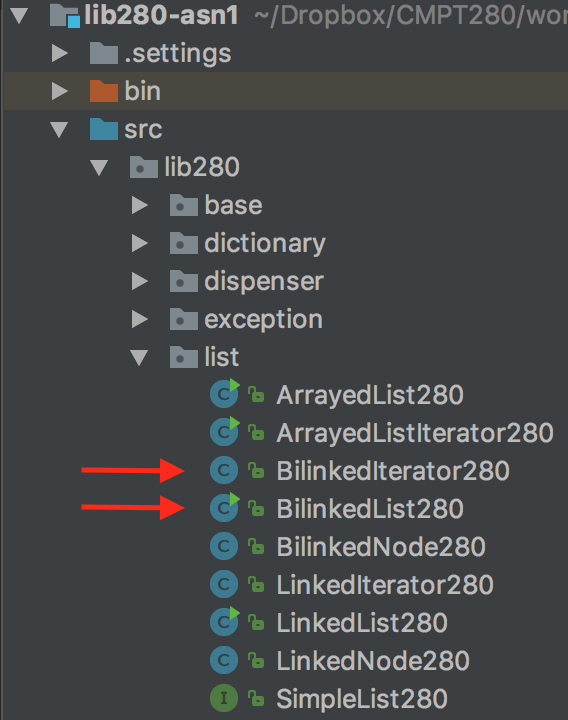
\includegraphics[width=.9\columnwidth]{figures/lib280.png}

\column{.5\textwidth}
\begin{itemize}
\item Things look nearly identical in Eclipse.
\item Important files for Asn1 are \BlistJ{} and \BiterJ{}
\item Definitely ignore the other packages for now.
\item Be aware of the other classes in \texttt{lib280.list} and their relationships to the bi-linked list classes.
\end{itemize}

\end{columns}

}


\frame{
\frametitle{Importing \libasn{} Lib280}
\begin{itemize}
\item Demonstration of how to create a project that references lib280.
\item Follow the part 3 of the self-guided tutorial from the website.
\end{itemize}
}

\section{Overview of Assignment 1}


\frame{
\frametitle{The actual questions}
\framesubtitle{Question 1}
Hints and Reminders;
\begin{itemize}
\item Don't forget to initialize the elements of the array \texttt{piratesByRank} in the given code.
\item The \texttt{Crew.java} class is given.  You don't have to write it yourself.
\item You only have to write a \texttt{main()} program finds that out determines much money jack pays in salary \textbf{per sack of grain} plundered by his crew members of each rank.
\end{itemize}
}

\begin{frame}[fragile]
\frametitle{The actual questions}
\framesubtitle{Question 1}
In this question you need to make an array of lists, conceptually:
\begin{center}
\begin{tikzpicture}[
llnode/.style={draw,rectangle split, rectangle split horizontal, rectangle split parts = 2, rectangle split part fill={structure.fg!50, white},anchor=west}
]
\draw (0,0) grid (1,5);
\node[llnode] (A1) at (3,0.5) {};
\node[llnode] (A2) at (4,0.5) {};
\node[llnode] (B1) at (3,1.5) {};
\node[llnode] (B2) at (4,1.5) {};
\node[llnode] (B3) at (5,1.5) {};
\node[llnode] (B4) at (6,1.5) {};
\node[llnode] (C1) at (3,2.5) {};
\node[llnode] (C2) at (4,2.5) {};
\node[llnode] (C3) at (5,2.5) {};
\node[llnode] (E1) at (3,4.5) {};
\node[llnode] (E2) at (4,4.5) {};
\node[llnode] (E3) at (5,4.5) {};
\node[llnode] (E4) at (6,4.5) {};
\node[llnode] (E5) at (7,4.5) {};
\draw (1.5, 0.15) rectangle (2.5, .85);
\draw[fill=structure.fg!50] (1.7, 0.2) rectangle (2.3, .5);
\node[anchor=south west,scale=.5] (H1) at (1.7, 0.5) {Head};

\draw (1.5, 1.15) rectangle (2.5, 1.85);
\draw[fill=structure.fg!50] (1.7, 1.2) rectangle (2.3, 1.5);
\node[anchor=south west,scale=.5] (H2) at (1.7, 1.5) {Head};

\draw (1.5, 2.15) rectangle (2.5, 2.85);
\draw[fill=structure.fg!50] (1.7, 2.2) rectangle (2.3, 2.5);
\node[anchor=south west,scale=.5] (H3) at (1.7, 2.5) {Head};

\draw (1.5, 3.15) rectangle (2.5, 3.85);
\draw[fill=structure.fg!50] (1.7, 3.2) rectangle (2.3, 3.5);
\node[anchor=south west,scale=.5] (H4) at (1.7, 3.5) {Head};

\draw (1.5, 4.15) rectangle (2.5, 4.85);
\draw[fill=structure.fg!50] (1.7, 4.2) rectangle (2.3, 4.5);
\node[anchor=south west,scale=.5] (H5) at (1.7, 4.5) {Head};

\draw[->] (.5, .5) -- (H1.west);
\draw[->] (.5, 1.5) -- (H2.west);
\draw[->] (.5, 2.5) -- (H3.west);
\draw[->] (.5, 3.5) -- (H4.west);
\draw[->] (.5, 4.5) -- (H5.west);

\draw[->] (2, .35) -- (A1);
\draw[->] (2, 1.35) -- (B1);
\draw[->] (2, 2.35) -- (C1);
\draw[->] (2, 4.35) -- (E1);

\draw[->] ($(A1)+(+.25,0)$) -- (A2.west);
\draw[->] ($(B1)+(+.25,0)$) -- (B2.west);
\draw[->] ($(B2)+(+.25,0)$) -- (B3.west);
\draw[->] ($(B3)+(+.25,0)$) -- (B4.west);
\draw[->] ($(C1)+(+.25,0)$) -- (C2.west);
\draw[->] ($(C2)+(+.25,0)$) -- (C3.west);
\draw[->] ($(E1)+(+.25,0)$) -- (E2.west);
\draw[->] ($(E2)+(+.25,0)$) -- (E3.west);
\draw[->] ($(E3)+(+.25,0)$) -- (E4.west);
\draw[->] ($(E4)+(+.25,0)$) -- (E5.west);

\end{tikzpicture}
\end{center}
\end{frame}


\begin{frame}[fragile]
\frametitle{The actual questions}
\framesubtitle{Question 1}In Java, have to cheat a bit to get around limitations of arrays of generic types to create an array of lists of \texttt{Crew} instances:
\begin{lstlisting}[basicstyle=\tt\tiny]
@SuppressWarnings("unchecked")    
LinkedList280<Crew> listArray[] = new LinkedList280[size];
//           ^^^^^^ Type parameter here!         ^^^ but not here!  
\end{lstlisting}
The \texttt{@SuppressWarnings("unchecked")} stops Java from complaining that this is unsafe.  It \textbf{is} unsafe, but only if you go out of your way. 

A type name without its generic type parameters provided is called a \textit{bare type}. 
\end{frame}




\frame{
\frametitle{The actual questions}
\framesubtitle{Question 2}


\begin{itemize}
\setlength{\itemsep}{1em}
\item Fill in the \cc{// TODO}s based on the method headers.

%\begin{center}
%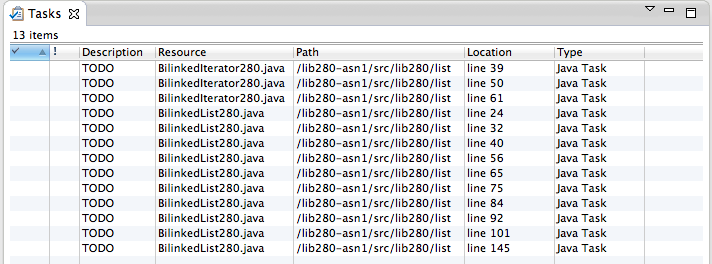
\includegraphics[height=.45\textheight]{figures/tasks.png}
%\end{center}

\item \textbf{ONLY} fill in the \cc{// TODO}s.  Do not change other code.\\ 
		(This is both easier and required.)
\end{itemize}


}


\frame{
\frametitle{The actual questions}
\framesubtitle{Question 2}

Tips and tricks: 

\begin{itemize}

\item The javadoc comments are how your javadoc comments should look on future assignments. 
	\begin{itemize}
		\item They are representative in terms of both appearance and quality.
	\end{itemize}

\item In general, good javadoc comments mean that IntelliJ will explain code to you. 
	\begin{itemize}
		\item Specifically, they'll explain the \lib{} to you.
	\end{itemize}

%\item With \cc{super}, some methods can be single statements. Some will be almost single statements.  Not just \cc{super}, though.  Using other methods is 
%	\begin{itemize}
%		\item good programming practice, and
%		\item easier.
%	\end{itemize}
%
\end{itemize} 

}



\frame{
\frametitle{The actual questions}
\framesubtitle{Question 3}
\begin{itemize}
\item Write regression tests for the new methods you wrote. 
\item Guidelines for writing tests can be found in the Topic 2 lecture notes.
\end{itemize}
}

\frame{
\frametitle{Policy reminder}
\begin{itemize}
	\item Late assignments are not accepted and will get a mark of 0. 
	\item Partial assignments that are handed in on time will receive partial credit. 
	\item You could hand in tests for question 3, but no implementations on question 2 and still get points for how good the tests are.  Black-box testing only requires that you know the interface, which you are given!
	\item \textbf{\underline{Please}} ask for help if you need it.  If you're stuck for more than 30 minutes, it's time to ask for help.  Help is available via email, in-person at help desk times, and through moodle forums.
\end{itemize}


}























\end{document}



